%===============
% Applicability
%===============

\chapter{Applicability of Different MVC Architectures for Web Applications}
\label{chap:webmvc}
In the previous two chapters, the \acl{mvc} pattern as well as technologies and techniques relevant to web application architectures have been presented. The challenges that result from applying MVC to web applications are discussed in this chapter by means of three defined criteria and four different MVC architecture variations.

\section{Evaluation Criteria}
In this section, three criteria --- \emph{data model complexity}, \emph{real-time model synchronization}, and \emph{data volume} --- are defined to help evaluating the applicability of different possibilities to implement \ac{mvc} in web applications. These criteria are accompanied by problems that have to be solved by an appropriate architectural design.

Some of the criteria are quantitative and can thus be evaluated objectively, such as \emph{Data Volume}. Others, such as \emph{Data Model Complexity}, are rather intangible and thus have a high interpretability. Therefore, examples are given to illustrate each criterion.

%=============================================================================
%=============================================================================

\subsection{Data Model Complexity} % gegeben
\label{sec:complexity}
Data model complexity is a criterion that cannot be measured objectively, and is also hard to define. It is an inherent problem for many domains that needs to be solved by an adequate web application architecture.

The complexity of a data model can best be illustrated by means of a relational database. The more the data model is normalized, the more complex it is. Normalization of data means to minimize redundancy and dependency. Normalized data often have cross references --- foreign keys in relational databases, object references in object--oriented programming languages and databases.

For Model--View--Controller based web applications, complex data models lead to a large number of Models and references between different Models. This can have challenges for the software design on the one hand, and for maintaining data consistency on the other hand.

\subsubsection{Examples}
A simple \emph{task application} with the only domain data being ``tasks'' has no high data model complexity. There usually is an additional Model for the users, but this never has to be managed on the client side. Users do not interfere with each other in this application, and they can only access their own tasks. A good example for an application of low data model complexity is \emph{Do It (Tomorrow)}\footnote{See \url{http://tomorrow.do/}}.

A project management application that manages users and roles, teams, projects, tasks and milestones and provides both an end-user as well as an administrator interface, has a high data model complexity.

\acl{icn} also is an illustrative example for web application with a complex data model. There are not only nested and interconnected Models, but also different data sources for the Models. \ac{rest} services can either be directly connected using Dojo, or they are accessed using the service layer of ICN as a proxy. In the latter case, Dojo interfaces with a service that acts as a REST API and redirects every request to the actual REST server after applying advanced business logic --- such as authentication and authorization. This can, for example, be used for \ac{sso}. Other data sources, such as the content repositories FileNet P8 and ContentManager, also have to be included. The fact that Content Navigator supports multiple repositories through \ac{sso} in one single interface leads to an even higher complexity. ICN is described in Chapter~\ref{chap:nexus} in more detail.
% separation of concerns, also in web app <-- ich hab keine ahnung mehr, was ich damit sagen wollte... =/

%=============================================================================
%=============================================================================

\subsection{Real-time Model Synchronization} % nfq
\label{sec:realtime}
In the area of web applications, the term \emph{real--time} is not comparable with ``real--time computing'', and should not be mistaken for it. A web application that supports real--time Model synchronization makes sure that changes to a server-side Model, which are taken by one client instance, are immediately pushed to all other client instances, too. Neither are those clients required to reload the page, nor do they have to request the updates themselves.

In opposition to this situation, the classic \emph{pull} mechanism is usually built as a \gls{timer}. A timer is a (JavaScript) function that gets executed periodically, for example ``every 5 minutes'', and pulls updates from the server to the client. For real-time Model synchronization, \emph{pull} can no longer be the technique of choice, as there might happen changes to a Model in between two executions of the timer. Instead, there are two possiblities for the server to notify the client of changes:
\begin{itemize}
	\item \emph{\gls{comet}}\label{term:comet} is an umbrella term for a set of techniques that allow low-latency data transfers in web applications. Two of them are commonly used: \emph{long polling} and \emph{forever frame}.

	Long \gls{polling} is ``a technique that optimizes traditional polling to reduce latency.''~\cite{schiemann07b} Whereas traditional polling means to send requests in defined time frames (for example ``every 15 seconds'') and to get an immediate response, long polling is not responded to until there actually \emph{is} something to respond with (e.g. updated data). This kind of request is also called long-running request. As soon as the HTTP respond returns, it is processed on the client, and another long-running request is sent immediately. The same happens if there is a timeout. Long polling makes use of the \pathname{XmlHttpRequest} JavaScript object.

	The ``forever frame'' is a different approach: an iframe\footnote{An \gls{iframe} (\emph{inline frame}) is an \ac{html} element that makes it possible to embed an \ac{html} document into another one.} is used to incrementally receive data, based on an \ac{http} 1.1 feature called \emph{chunked encoding}, as described by \citeasnoun{schiemann07a}. Using one single, long-lived \ac{http} request, data can be received whenever necessary, as they are sent in chunks. The connection is not closed until the server decides to close it.

	Both of these approaches --- and in general every Comet technique --- work asynchronously. This is essential for web applications that require real-time data synchronization, as user interaction would otherwise be blocked. On the server this problem can be solved using non-blocking \acs{io} or threads.

	There are Comet implementations for most JavaScript frameworks, such as \emph{cometD} for Dojo\footnote{See \url{http://cometd.org/}} and the comet plug-in for jQuery\footnote{See \url{http://archive.plugins.jquery.com/project/Comet}}.

	\item The new HTML5 \acp{api} provide the possibility to create long-lasting \ac{tcp} sockets in the browser, called WebSockets. Using a WebSocket, a permanent, duplex connection can be established to the server. Updates that happen on the client can be sent using this socket, and changes that are made on the server (or pushed to the server using other client instances) can be received.

	This concept is especially useful if combined with Web Workers, so that the socket is not blocking any user interaction or other application functionality.

	The great advantage over the \emph{forever frame} technique is that WebSockets work in both directions: not only can the server send information to the client, the client can also send additional information to the server (for example to abort the running request and send a different one).
\end{itemize}

\subsubsection{Examples}
Web-based communication tools, for example instant messaging programs, serve as good examples for the real-time criterion. The chat tool integrated in many of Google's products, \emph{Google Chat}, uses push techniques. Which techniques are used exactly is not publicly documented, but with respect to Google's leading role\footnote{Amongst others, Google develops the open source JavaScript engine V8, contributes to the WebKit HTML rendering engine and is part of the W3C (the comittee that develops web standards such as CSS and HTML).} in web technology development, it can be assumed that Google Chat uses WebSockets if available, and Comet techniques otherwise.

Other typical applications for a real-time synchronization scenario are collaboration tools. Google Docs\footnote{Now part of Google Drive, see \url{https://drive.google.com/}}, for example, is an online office suite that provides spreadsheets, documents, presentations and more. These documents can be edited by multiple users in real-time, which means you can see the changes another user makes right as he types, and vice-versa.

%=============================================================================
%=============================================================================

\subsection{Data Volume} % throughput; nfq
\label{sec:datavolume}
This criterion describes the volume of data a web application has to process. Data volume is critical to application speed and responsiveness.

It is assumed that the data volume described here has to be processed \emph{on the client}. In other words, the user has to get in contact with these data in some way, either by creating, manipulating or viewing them.

High data volumes are causing two significant problems that can slow down a web application:
\begin{itemize}
	\item Long network transfer times force the user to wait for data before he can work with the application. 
	\item A large amount of data in the browser memory can cause bad performance in older browsers or on older machines.
\end{itemize}

Both problems lead to bad usability of the web application. To solve these problems, network traffic between the application's client-side and server-side has to be reduced to a minimum. There are several techniques to achieve this, including the following two:
\begin{description}
	\item[Lazy loading] is one approach to reduce both network traffic and the amount of data being held in browser memory. It is based on the assumption that not all the data have to be present on the client at once. Lazy Loading means loading data ``on demand''. Usually, it is implemented using some sort of prediction strategy which predicts what data will have to be loaded next. This way, the user does not need to actively request additional data.

	Lazy Loading needs a client-side Model, or at least an instance that manages the state of data that are already loaded, so it can be determined which parts of the data still need to be loaded.

	Although the actual Model may be quite large on the server, lazy loading keeps it as small as possible on the client and leads to a more performant application.
	\item[Caching] can be leveraged on different network nodes, for example using a proxy, web server or browser cache. But also web applications can implement caching. Using the HTML5 \emph{localStorage} \ac{api}, data can be made persistent on the client side using an associative data model\footnote{Associative arrays map a certain value to a key, and are therefore also called ``key--value stores'' or ``dictionaries''.}. Other storage \glspl{api}, such as IndexedDB or WebSQL can be used too, but are not as widely supported by browsers as localStorage.

	% Caching is only one use case for client-side data persistence, but the one relevant in this context. Along with the use of the localStorage \ac{api}, a cache strategy has to be used to not fill the store with obsolete and dispensable data.
\end{description}

In addition to the techniques used for the data volume of Models, also the data volume of source code can be reduced. This can be achieved by packaging code into logical, independent \emph{modules}. In opposition to server-side programming languages like Java, \gls{ruby}, Python or C++, JavaScript --- as of version ECMA-262 --- does not provide a way to import and use modules.

A solution to this is \ac{amd}\label{term:amd}\footnote{See \url{https://github.com/amdjs/amdjs-api/wiki/AMD}}, an API for packaging code into modules and loading them asynchronously, on demand. It is supported by RequireJS, Dojo as of version 1.7 and other JavaScript frameworks and libraries.

The amount of data to transfer from the server to the client is usually smaller if using AMD, as only the parts of the application are loaded that are really needed. This leads to shorter loading times. Additional components, which were not needed at the initial loading of the application, can be loaded as their functionality is requested (known as ``\ac{jit}'').

\subsubsection{Examples}
\emph{Twitter}\footnote{Twitter is a web application to exchange short messages, so-called \emph{Tweets}, with other people (\emph{Followers}) who have subscribed to you.} is an application with very high data throughput: 200 million Tweets were sent per day as of November 1st, 2011 (over 2300 per second)\footnote{See \url{https://dev.twitter.com/discussions/3914}}. Although every user can only see a small fraction of these, the Twitter stream cannot show \emph{all} Follower's Tweets at once. Therefore, the Twitter web application as well its Android and iOS applications all support lazy loading for the list of Tweets. It only loads a limited number of Tweets on initial page load, but loads additional (older) ones when the user scrolls down the page. Twitter shows a loading animation (see Figure~\ref{fig:ll}), although this animation should not be seen by users, due to predictive loading (Tweets are loaded \emph{before} the user reaches the bottom of the page). To make this screenshot possible, the internet connection was shut down temporarily.

\begin{figure}[H]
	\centering
	
\includegraphics[width=14cm]{screens/twitter_ll.png}
	\caption{Lazy loading on Twitter, indicated by a loading animation}
	\label{fig:ll}
\end{figure}

%\newpage
A second illustrating example for handling of high data volumes is \emph{Backbone.js}. This is a JavaScript framework for structuring client-side web applications according to an adaptation of the \acl{mvp} pattern. It uses RESTful calls via \ac{ajax} to synchronize its client-side Model with the server. These calls can be replaced by a localStorage adapter\footnote{See \url{https://github.com/jeromegn/Backbone.localStorage}}, so that localStorage is employed as the persistence layer.

Models in Backbone.js are single objects that keep a record of domain data. To store more than one record, a Collection is used\footnote{This is a matter of terminology. ``Model'' often refers to a whole set of records, but the Backbone.js developers decided to use this term for a single instance and the term ``Collection'' for multiple instances.}.
Backbone.js allows to assign the persistence storage on a per-Collection basis.

Using two different Collections of the same Model allows the developer to implement a cache mechanism for Model data. One Collection is used to connect to the actual persistence layer, for example a \gls{rest} server, whereas the other one connects to the localStorage. If Model data are requested, the application can first look for them in the localStorage Collection; if they are not present there, they are requested from the REST Collection and copied to the localStorage Collection for caching. As in every cache mechanism, the implementation has to make sure that the cached data are up--to--date.

Listing~\ref{lst:localstorage} shows the definition of a ``Person'' Backbone.js Model including default values and input validation. The ``People'' Collection of ``Person'' Models is tied to the localStorage \ac{api} for data persistence.
To illustrate the usage of Models and Collections in Backbone.js, a ``Person'' is instantiated and saved into the Collection.


\begin{listing}[H]
\begin{minted}[linenos=true,frame=no]{javascript}
var Person = Backbone.Model.extend({
  defaults: {
    salutation: "Mr.",
    age: 18,
    children: []
  },
  validate: function(attributes){
    // If validate() returns a string, Backbone throws an error
    if(attributes.age < 0) {
      return "You can't be negative years old";
    }
    if(name === undefined)
      return "You need to have a name";
    }
    // This requires the jQuery library
    if(!$.inArray(attributes.salutation, ["Mr.", "Mrs.", "Ms."])) {
      return "You need to have a proper salutation";
    }
  }
});

var People = Backbone.Collection.extend({
  // Save in the localStorage repository "People"
  localStorage: new Backbone.LocalStorage("People"),
  // Use the Model defined above
  model: Person
});

var bruce = new Person({
	name: "Bruce Wayne",
	age: 32
});

var age = bruce.get("age"); // 32
var name = bruce.get("name"); // "Bruce Wayne"
var salutation = bruce.get("salutation"); // "Mr."
var children = bruce.get("children"); // []

var localCollection = new People();
localCollection.push(bruce);
\end{minted}
\caption{Backbone.js Model and Collection using localStorage for persistence}
\label{lst:localstorage}
\end{listing}

%=============================================================================
%=============================================================================
%=============================================================================
%=============================================================================
\newpage
\section{MVC Architectures in Web Applications}
\label{sec:mvcwebarch}
The Thin Client and Rich Client architectures introduced in Section~\ref{sec:clientserver} are general descriptions of frequently implemented web application architectures, independently of \acl{mvc} or any other architectural pattern. If in the software engineering process a pattern of the MV* family is chosen for a web application architecture, some decisions are yet to be made. There are several ways to implement \acl{mvc} on client as well as on server side, as the components can be distributed on both network nodes differently. This section discusses various solutions, along with synchronisation strategies and possible implementations.

\subsection*{Controller and Router}
\label{term:router}
It is necessary to clarify the terms ``Controller'' and ``Router'' in this section to avoid misunderstandings. The design pattern \emph{Front Controller} or \emph{\gls{router}} (both terms describe the same pattern) were already introduced on page~\pageref{term:frontcontroller}. According to \citeasnoun[p. 105]{osmani}, routers are ``neither a part of MVC nor present in every MVC-like framework''. This is definitely true for Model--View--Controller as a pattern, but when implementing it in a 2--tier web architecture, the router is an inevitable part, as it is a Controller ``that handles all requests for a Web site'' \cite[p. 344]{poeaa}.

The Router has a responsibility that is originally assigned to a regular MVC Controller: it reacts on user input. On thin clients, the only user input recognizable by the application is coupled to HTTP requests. This includes navigation on the one hand (the user clicking on hyperlinks) and submitting form data on the other hand. Both actions are tied to URLs, so the processing of the according requests --- which are in the responsibility of a Controller --- is done by a Router.

An excellent example for this is Model 2, a Java EE implementation of MVC, which uses a Servlet as the Front Controller (see page~\pageref{term:model2}). This Servlet chooses actions to take and the View (JSP) to display based on the URL, which is both a Router's and Controller's task.

As a conclusion, it can be assumed that routing in web applications is part of the server--side Controller, which is the reason why the diagrams in the following section do not show a distinct Router component. The first three MVC web architectures handle routing on the server, as they all include a server--side Controller. %Only the last architecture variation, \emph{Rich Client MVC Architecture}, handles routing on the client side using JavaScript.

\subsection*{On Applicability}
The applicability of the presented MVC architectures is assessed on the basis of the previously defined criteria. For each of the four architecture variations, a table is given to evaluate the applicability of an architecture with respect to one of the three criteria. For each criterion, the result can be
\begin{itemize}
	\item \emph{Yes}, which means that this architecture is suitable for web applications with the respective requirement, as most arguments are in favor.
  %It does not mean, however, that this is true in all possible cases; there may be applications that work better with a different architecture.
	\item \emph{No}, which means that this architecture is not suitable for web applications with the respective criterion, according to most of the presented arguments.
  %There are exceptions to this, too.
	\item \emph{Depends}, which means that there are balanced arguments speaking for and against the applicability of this architecture.
  \item There are always exceptions to these evaluation results.
\end{itemize}

The choice of the right architecture for an application depends on many factors. The applicability tables created here are not absolute, but provide an objective (as in ``supported by arguments'') basis to compare the four architecture variations.

%=============================================================================
%=============================================================================

\subsection{Server Side MVC Architecture}
\label{sec:thinclientmvc}
% General
The classical and most simple solution is to implement the \ac{mvc} stack completely on the server side. This would be the case in a Thin Client as described in Section~\ref{sec:thinclient}.

The View in this variation is usually an \ac{html} file, created using an \ac{html} preprocessor or a templating language\footnote{A templating engine is a software that processes a text file, replacing placeholders with actual values that are valid for a given situation. In addition to placeholders, constructs of programming languages --- like conditionals and loops --- can often be used too, hence the term \emph{templating language}.}. It gets preprocessed on the server, is then sent to the browser and not modified after that. The user interacts with the MVC application through the web browser, which is why there is no real client--side View, but only the \ac{dom}.

When using an object-oriented programming language on the server, the Models can be implemented interfacing an \gls{orwrapper} or the \ac{api} to an \gls{oodb} like MongoDB or CouchDB. A Model then would basically be a class that utilizes \ac{crud} methods. In procedural programming languages, the Model usually is the database itself. It can be manipulated and queried directly from the programming language, for example using the \ac{sql}.

The Controller is the application code inside the View, or included in the View through external files. It is code that decides what actions to take and with which values to fill the template's placeholders, depending on application state and user input.

Following the description above, the components in a \emph{Server Side MVC Architecture} can be very closely coupled, which contradicts the idea of \emph{Separation of Concerns}. Frameworks, such as the two described below, try to enforce decoupling.

\subsubsection{Structure}
% Structure
Figure~\ref{fig:thinclientmvc} shows the architecture of a full server-side \ac{mvc} web application.
\begin{figure}[H]
	\centering
	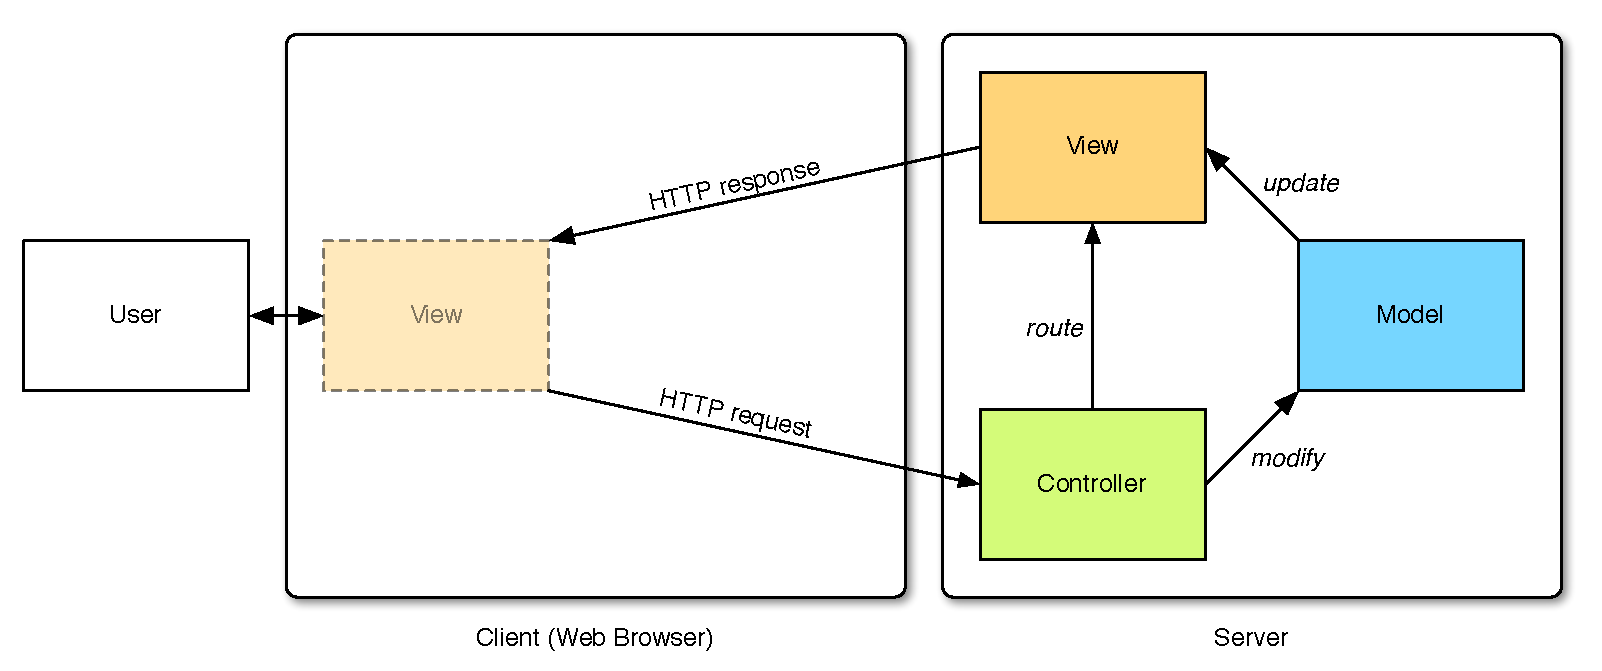
\includegraphics[width=16cm]{images/thinclientmvc.pdf}
	\caption{Structure of a Server Side MVC Architecture}
	\label{fig:thinclientmvc}
\end{figure}

The diagram reflects the sequence of control in this \ac{mvc} scenario. It is assumed that the server-side View is bound to a \ac{url}, and thus is the \ac{html} document to receive. Loading of a \ac{url} is always initiated by the user through the web browser.

The client-side View is displayed slightly transparent, as it is not a real \ac{mvc} View that gets data from a Model and performs actions through a Controller. It is the displayed version of the web page that was loaded in the browser, and it acts as a mediator between the user and the server (following \glspl{url} after the user clicks on links and displaying a web page after it is received). In later presented architectures, the Controller is mapped to a \gls{url} and invoked by the client-side Controller, instead of by the server-side View.

\subsubsection{Implementations}
% Implementations
Common implementations for this variant include \ac{mvc} frameworks for server-side programming languages:
\begin{description}
  \item[Struts] is an open source framework for building web applications using \ac{jee}. It implements a \emph{Model 2} architecture, as described in Section~\ref{sec:thinclient}. Struts uses a Servlet as the Front Controller to route requests to the actual Controller, which is responsible for a certain request. It responds with JSPs as Views and uses JavaBeans as Models.\footnote{See \url{http://struts.apache.org/}}

	\item[Ruby on Rails]--- or just \emph{Rails} --- is a \ac{mvc} web application framework for the Ruby programming language. It can make use of a variety of templating systems (eRuby, HAML and others) to construct Views. For the Models, Rails uses an object-relational wrapper on top of a relational database (such as MySQL, SQLite, DB2, and Oracle), but extended through plug-ins it can also use object databases for persistent storage of domain data.

	\gls{rails} ships the JavaScript framework \emph{Prototype}, which makes it possible to build \ac{ajax} applications using Rails as the backend, but Rails itself is a pure server-side \ac{mvc} framework.\footnote{See \url{http://rubyonrails.org/}}
\end{description}

\subsubsection{Applicability}
\begin{table}[H]
	\centering
	\begin{tabular}{l l}
\rowcolor{lightgray}
Criterion & Applicability\\
Data Model Complexity & \emph{Yes}\\
Real-time Model Synchronization & \emph{No}\\
Data Volume & \emph{No}\\
	\end{tabular}
	\caption{Applicability of a Server Side MVC Architecture}
\end{table}
The \emph{Server Side MVC Architecture} can be used for applications with a complex data model. As the pattern components reside completely on the server side, maintenance is easier to perform than if it was distributed. \ac{mvc} frameworks such as Struts, Spring, FLOW3, Rails and Synfony offer data modelling possibilities that are powerful enough to reproduce even very complex data models.

It is not suitable for real-time Model synchronization. Once sent to the client, the page cannot be updated --- it remains static. Providing real-time updates, or even non-real-time updates, would require a client-side mechanism to request and process subsequently sent data. Such mechanism is not present in a Server Side MVC architecture.

High data volume turns out to be a problem for this architecture, too. As data cannot be fetched after the site is loaded, all data that the user could want to process have to be loaded initially, and again with every navigational action the user might take. This results in high network traffic.

%=============================================================================
%=============================================================================
\newpage
\subsection{Distributed Controller MVC Architecture}
\label{sec:distcontr}
% General
The first change that can be made to the full server-side \ac{mvc} is to push the Controller to the client-side. This does not mean that there is no Controller on the server anymore, but its responsibility is reduced in comparison to a full server-side one. Thus, this \ac{mvc} web application architecture can be called \emph{Distributed Controller MVC Architecture}.

In Server Side MVC Architecture applications, navigational actions are bound to different pages. Refreshing a View requires to refresh the web page, and manipulating the Model is usually bound to calling a URL with POST or GET parameters --- which is the Controller's task.

In Distributed Controller MVC applications, the navigation is not only bound to different \emph{pages}. Still, pages can be accessed through the \ac{url} and lead to different main areas of the application. This task of routing is done by the server-side Controller\footnote{See p. \pageref{term:router} for more information on the connection between \emph{Controller} and \emph{Router} in web-based MVC applications.}.
The client-side part of the Controller, on the other hand, is encorporated by the possibility to interact with the web application \emph{without} changing the page (and thus loading a new \ac{url}) each time. It is realized as JavaScript code running in the browser, which is capable of handling minor navigational patterns within the page and delegating Model manipulation to the server--side Controller using \ac{ajax}. These tasks can include \gls{lazyloading} of content when scrolling or the creation of popup windows to display more detailed data.

Manipulations on the Model are initiated from the client-side Controller using an AJAX call, but are carried out by the server-side Controller code. This is usually a Servlet or a script, as described for Server Side MVC on page~\pageref{sec:thinclientmvc}. The server--side Controller needs to be able to analyze the AJAX request and act accordingly. The \emph{Distributed Controller MVC Architecture} does not maintain a client-side Model.

% Structure
\subsubsection{Structure}
The following architectural diagram (Figure~\ref{fig:distcontr}) illustrates the distributed Controller component.
\begin{figure}[H]
	\centering
	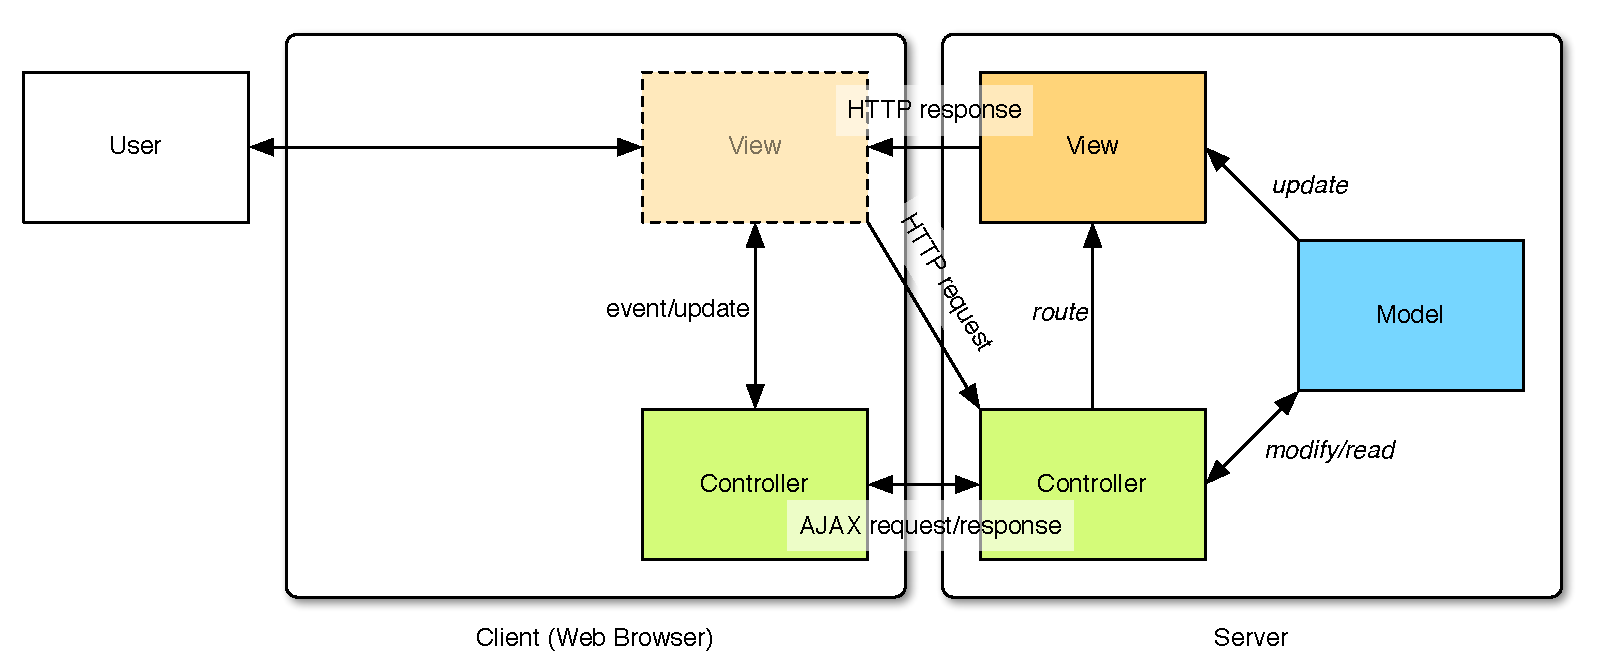
\includegraphics[width=16cm]{images/distcontrollermvc.pdf}
	\caption{Structure of a Distributed Controller MVC Architecture}
	\label{fig:distcontr}
\end{figure}

% Implementations
\subsubsection{Implementations}
The \gls{twitter} web application implements a Distributed Controller MVC Architecture, which is described by \citeasnoun{selvitelle}.

The application's main areas (``Home'', ``Connect'' and ``Discover'') as well as users' profiles have their own \acp{url}. Thus, the application has a server-side Controller. However, there is a lot of functionality that can be used without switching pages.

For example, when looking at a Twitter stream (or a search), you can scroll down to the bottom of the page, and additional (older) \glspl{tweet} are loaded. The respective event, in natural language ``the user scrolls to near the bottom of the page'', is processed by a client-side Controller, which then sends an \ac{ajax} request to the server and inserts the results (more Tweets) into the View (the list of Tweets, or \emph{stream}). This can be examined by logging the HTTP activity of Twitter.

According to \citeasnoun{venners}, the Twitter web application is based on Ruby on Rails as the server-side MVC framework.
For the client-side, there is no MV* framework used. Twitter only includes the jQuery JavaScript library, which is used for event handling and AJAX requests (client-side Controllers). This is proven by the JavaScript source code used by Twitter.

\subsubsection{jQuery Example}
To illustrate the interaction of client-side and server-side Controller, the following listings show how data from a form can be made persistent on the server without reloading the page. A simple task application using the JavaScript library \emph{jQuery} serves as an example.

\begin{listing}[H]
\begin{minted}[linenos=true,frame=no]{html}
<form>
  <input type="text" />
  <button type="submit">Add new Task</button>
</form>	
<ul>
  <li>Wash the dishes</li>
  <li>Do laundry</li>
  <li>Grocery shopping</li>
</ul>
\end{minted}
\caption{Task list HTML skeleton (View)}
\label{lst:taskhtml}
\end{listing}

The HTML skeleton in Listing~\ref{lst:taskhtml} contains a form with an input text field and a submit button, respectively. Also, it contains a list of items that represent already existing \emph{tasks}.

\begin{listing}[H]
\begin{minted}[linenos=true,frame=no]{javascript}
$('form button').click(function (event) {
  event.preventDefault();
  $.ajax({
    url: "newtask.php",
    data: {
      task: $('form input').val()
    }
  }).done(function() {
    $('<li>').html( $('form input').val() ).prependTo('ul');
    $('form input').val('').focus();
  });
});
\end{minted}
\caption{JavaScript-based client-side Controller for the task list}
\label{lst:taskjs}
\end{listing}

The JavaScript code in Listing~\ref{lst:taskjs} represents the client-side part of the Controller. An anonymous function is registered as a callback for the \emph{click} event of the form's submit button. In the callback itself, the default behaviour (that would be to submit the form) is prevented using \code{event.preventDefault();}. Then, an \ac{ajax} request is sent to the \ac{url} \pathname{newtask.php}, providing the text inside the form's input field as a parameter. By default, this is an asynchronous call using the \ac{http} GET method.

When the call returns successfully, another callback (the anonymous function inside the \code{\$.ajax().done()} invocation) adds the new task as a list item on top of the existing list. It then clears the input field and gives the keyboard focus back to it.

The \ac{php} code of the server-side Controller is not listed here. It would typically insert the given task into a database and return a unique ID, which then could be processed on the client.

% Twitter benutzt eine Mischugn aus diesem und dem nächsten

\subsubsection{Applicability}
\begin{table}[H]
	\centering
	\begin{tabular}{l l}
\rowcolor{lightgray}
Criterion & Applicability\\
Data Model Complexity & \emph{No}\\
Real-time Model Synchronization & \emph{Yes}\\
Data Volume & \emph{Depends}\\
	\end{tabular}
	\caption{Applicability of a Distributed Controller MVC Architecture}
\end{table}
The Distributed Controller MVC Architecture makes more use of client-side programming and thus is applicable for web applications that require more dynamicity on the client-side than the Server Side MVC Architecture.

The fact that this MVC distribution allows additional data loading without maintaining a client-side Model makes it a good choice for simple data structures. Complex Models, on the other hand, are harder to implement using the Distributed Controller MVC, as the missing client-side Model makes it impossible to manage data in a structured way. It is sufficient for the Twitter web application, as its data model is rather simple.

The client-side Controller allows loading data at any time, so it is possible to build applications with real-time data synchronization capabilities using a Distributed Controller MVC Architecture (although synchronization happens only from the server to the client in this case, as the client does not maintain a Model).

High data volumes can also be handled by this architecture. Using techniques like lazy loading, as Twitter does, data can be loaded on demand. However, depending on the amount of data and if the data should further be processed, an architecture with a client-side Model may be the better solution.

%=============================================================================
%=============================================================================

\subsection{Synchronized Model MVC Architecture}
% General
The next step towards a Rich Client is to bring the Model into the browser. In opposition to the Controller in the architecture discussed before, there is no distribution of Model responsiblity across the network nodes. Instead, the client-side Model is a copy, or an excerpt, of the original, server-side Model. The one in the browser is the operating Model --- all client-side manipulations are executed on the client-side Model. The server-side Model is used for persistence, which requires a synchronisation strategy between client and server.

The synchronisation strategy and possibilities of the client-side Model highly depend on what the Model represents.
\begin{itemize}
	\item If the client-side Model is an \emph{exact copy} of the server-side one (i.e. it keeps all the data that are also contained on the server-side), all Views and Controllers can directly interact with this exact Model. Synchronisation can happen
	\begin{itemize}
		\item periodically, i.e. after a defined amount of time (``timeout'')
		\item on special actions, e.g. manipulation of the client-side Model
	\end{itemize}
	It is recommended to only synchronize the differences between the client and server, usually called ``delta''.

	\item The client-side Model can also be only a \emph{partial copy} of the server-side one. By keeping track of which part of the data is already present on the client, data can be efficiently transferred from and to the server. This is preferred for high volumes of data. 

	The synchronisation strategies are the same as described above. Lazy loading can best be implemented using a partial client-side Model.
\end{itemize}

% Structure
\subsubsection{Structure}
\begin{figure}[H]
	\centering
	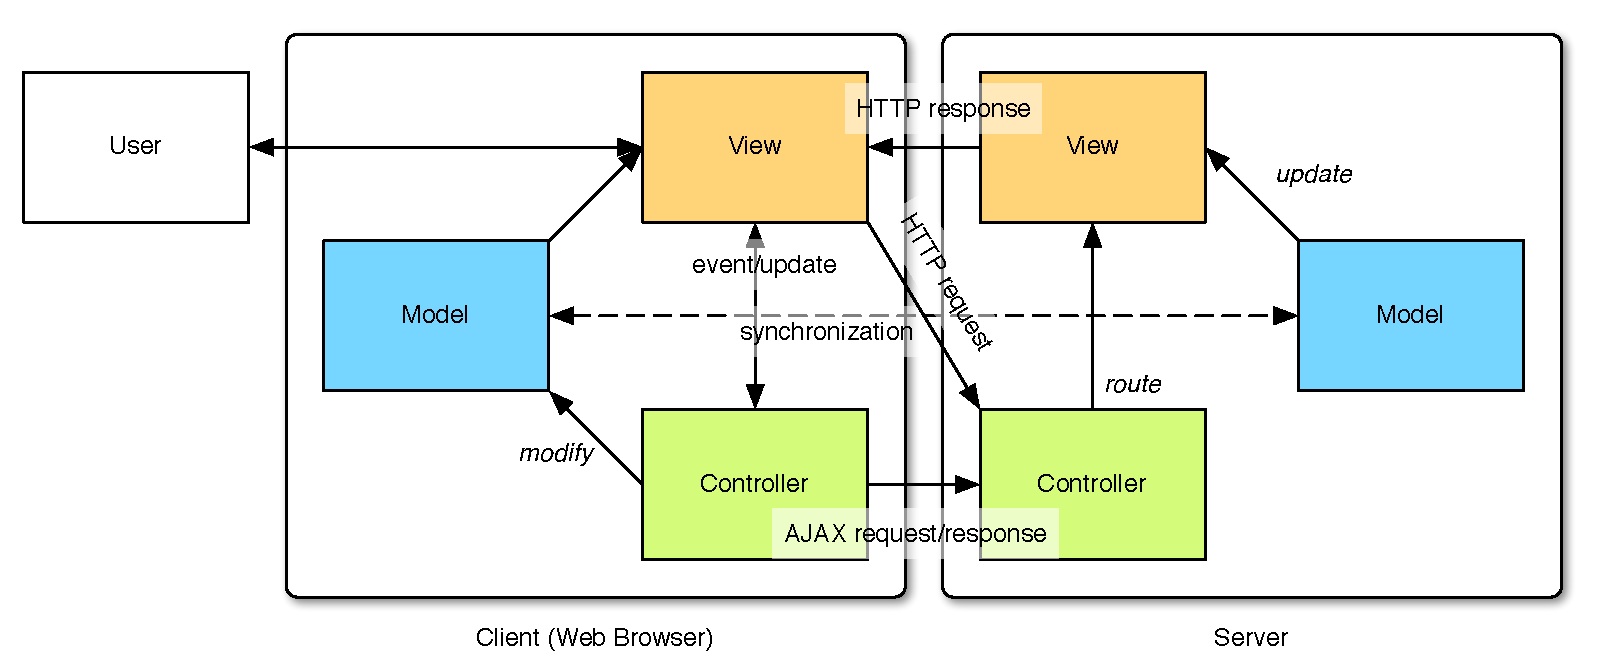
\includegraphics[width=16cm]{images/syncmodelmvc.pdf}
	\caption{Structure of a Synchronized Model MVC Architecture}
	\label{fig:syncmodel}
\end{figure}

In this architectural diagram, the synchronization between the client-side and server-side Models is illustrated using a dashed line.

\subsubsection{Implementations}
Once Model synchronisation is part of the architecture, a client-side MV* framework is often used to structure the JavaScript code; this is especially useful, as basic functionality for synchronisation and data I/O do not have to be implemented manually, but are provided by most frameworks.

There are a lot of examples that make use of the Backbone.js framework. The open-source social network \emph{Diaspora}\footnote{See \url{https://joindiaspora.com/}}, for example, uses Ruby on Rails as a server-side MVC framework, and in parallel Backbone.js on the client-side. Although Ruby on Rails follows MVC and Backbone.js is built after MVP, these two frameworks work together well.

Backbone.js Models can directly synchronize with Rails Models without any further transformations, as they can be configured to use the same JSON format for data exchange.

One can argue that the presence of a complete MV* triad on the client makes the server-side Controller obsolete: it is no longer needed to manipulate the server-side Model. This is correct for completely client-sided MV* applications, as described in the next section (\emph{Rich Client MVC}). Rich Client MVC applications are one-page applications, which means that their user interface and routing is handled completely using JavaScript. But in applications following the Synchronized Model architecture, both routing and initial creation of the user interface happens on the server-side.

Another advantage of the server-side Controller is the fact that multiple front-ends can be built to collaborate with the server. In addition to the web client, mobile clients that follow a thin client paradigm --- for example for performance reasons --- can make use of the completeness of server-side MVC.

\subsubsection{Applicability}
\begin{table}[H]
	\centering
	\begin{tabular}{l l}
\rowcolor{lightgray}
Criterion & Applicability\\
Data Model Complexity & \emph{Depends}\\
Real-time Model Synchronization & \emph{Yes}\\
Data Volume & \emph{Yes}\\
	\end{tabular}
	\caption{Applicability of a Synchronized Model MVC Architecture}
\end{table}

% Complexity
The parallel structure of a Synchronized Model MVC Architecture makes the handling of comples data models difficult. Data can be changed on two different points in the application: on the client, using the client--side Controller, and on the server, using the client--side Controller to send an AJAX request to the server--side Controller, which then modifies the Model. Of course it is possible to efficiently resemble complex data models with this architecture variation, but with a lot of Models and cross-references included, it is possible that the structure becomes intransparent.

%Due to the parallel architecture of Synchronized Model MVC, handling complex Models may need high effort, as suitable Views have to be built on both the client-side and server-side. Changes have to be made on both sides, too. A possible solution would be to implement modules in a format that can be used by both the client-side and the server-side code. This can include a templating language understood by both a JavaScript framework and the programming language used on the server. Another approach is to use JavaScript for both server and client code, for example using the server-side JavaScript platform \emph{Node.js}\footnote{See \url{http://nodejs.org/}}.

% Real-time
The synchronization of the Model makes applications with real--time snychronization possible, even for more complex data structures. Using the techniques described as \emph{\gls{comet}} and WebSockets on page \pageref{term:comet}, every synchronization strategy can be implemented, whether the client-side Model is a complete or only a partial copy of the server-side Model.

% Data Volume
This architecture is suitable for processing high data volumes, for the same reason as it is suitable for applications that require real-time data synchronization. As the Model is synchronized between client and server, it is possible to only load the required data onto the client-side and load additional data subsequently, on demand.

%=============================================================================
%=============================================================================

\subsection{Rich Client MVC Architecture}
The Rich Client MVC Architecture is described as  ``RIA Architecture''\glsunset{ria}\footnote{RIA is short for \emph{Rich Internet Application}. The term can be used for rich web clients, but it usually describes applications developed with Adobe Flash or Flex, see Section~\fullref{sec:terminology}} by \citeasnoun{steele}. It places the whole set of Model, View and Controller on the client-side, while only a Model stays on the server-side.

What distinguishes this variant from the \emph{Synchronized Model MVC Architecture} is that there is no server-side View or Controller anymore. Of course, there is an entry point to the application needed. This is usually an almost empty \ac{html} file that only contains a skeleton and references to additional resources, such as JavaScript, CSS and image files that have to be loaded subsequently. The user interface is being constructed on the client side, purely through JavaScript code.

\subsubsection{Structure}
\begin{figure}[H]
	\centering
	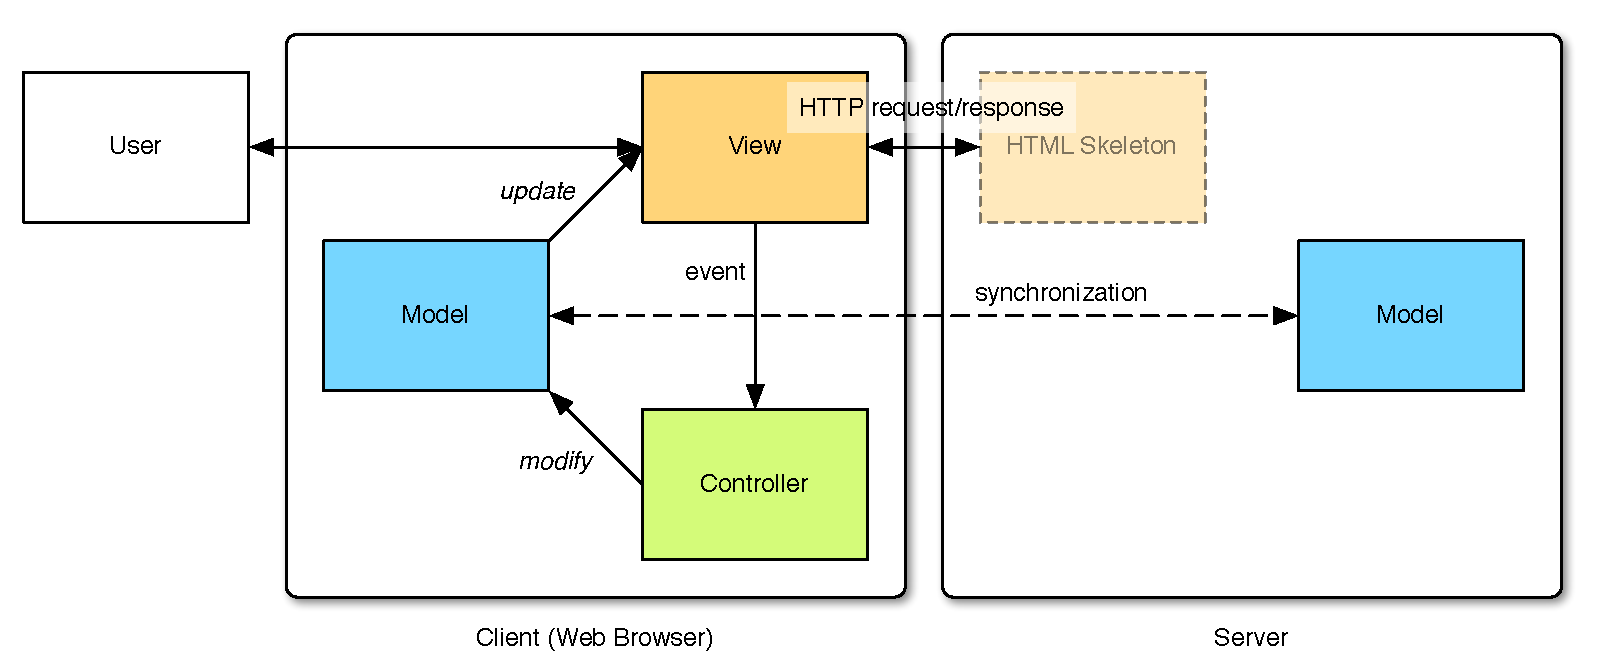
\includegraphics[width=16cm]{images/richclientmvc.pdf}
	\caption{Structure of a Rich Client MVC Architecture}
	\label{fig:richclientmvc}
\end{figure}

\subsubsection{Implementations}
The Dojo Toolkit\footnote{See \url{http://dojotoolkit.org/}} comes with a great variety of different modules and widgets (called \emph{Dijits}). Dojo 1.6\footnote{Please note that Dojo developed various \ac{mvc} approaches over time, and they differ quite a lot between versions 1.8 (the latest as of September 2012) and older ones. Dojo 1.7 provides the \pathname{dojox.mvc} package, but in this thesis, Dojo 1.6 is the version referred to, as it is the version used by \ac{ibm} \nexus\ at this time.} makes it possible to build pure client-side \ac{mvc} applications.

In Dojo, the Model is a Dojo Data Store, for example \code{dojo.store.Memory} and \code{dojo.data.ItemFileReadStore}. Using the \code{dojo.store.Observable} wrapper around the store, the Observer pattern can be established between View and Model. Views can be Dijits, either Dojo's own or custom ones. Controllers can be implemented as own modules, but often Controller code is put inside of the Dijit, which breaks with the \emph{Separation of Concerns} paradigm of \ac{mvc}.

Using the \code{dojox.data.JsonRestStore}, a RESTful web service can be connected to the client-side store, which allows data persistence on the \acs{rest} server and makes a Rich Client/Thin Server configuration possible.
Dojo's \ac{mvc} implementation is further discussed in Chapter~\fullref{chap:nexus}.

\subsubsection{Applicability}
\begin{table}[H]
	\centering
	\begin{tabular}{l l}
\rowcolor{lightgray}
Criterion & Applicability\\
Data Model Complexity & \emph{Yes}\\
Real-time Model Synchronization & \emph{Depends}\\
Data Volume & \emph{Yes}\\
	\end{tabular}
	\caption{Applicability of the Rich Client MVC Architecture}
\end{table}

A web application with a Rich Client MVC Architecture is able to handle complex data models. The most important requirement for this is a well-defined interface between the client-side and server-side Models. As the code to process and consolidate Model data is situated on the client-side only, even very complex domain data can be handled by this application architecture.

The Rich Client MVC architecture is suitable for real-time model synchronization, as long as a powerful modern web browser is used. This requirement has two reasons:
\begin{itemize}
	\item Depending on the complexity and the number of Models to synchronize, the \emph{Comet} technique described on page~\ref{term:comet} might not be feasible anymore. Too many iframes or pending requests in parallel can slow down the user interface. Using a modern browser that supports HTML5, WebSockets can be used for synchronization, which also allow more control over the data transfer.
	\item Due to the fact that the whole application is situated on the client-side, a lot of memory might be needed. Also, the execution time of JavaScript code can be slow if the JavaScript engine is not capable enough to run a full-fledged, desktop-level web application.
\end{itemize}

Regarding data volume, the same is true for Rich Client MVC as it is for a Synchronized Model MVC architecture.

%=============================================================================
%=============================================================================
%\newpage
\subsection{Comparison and Conclusion}

The results of the applicability evaluation are summarized in Table~\ref{tab:comparison}.

\begin{table}[H]
	\centering
	\begin{tabular}{l p{2.4cm} p{3cm} p{3cm} }
\rowcolor{lightgray}
MVC Architecture & Data\ Model Complexity & Real-time Model Synchronization & Data Volume\\
Server Side & \cellcolor{green}\emph{Yes} & \cellcolor{red}\emph{No} & \cellcolor{red}\emph{No}\\
Distr. Controller & \cellcolor{red}\emph{No} & \cellcolor{green}\emph{Yes} & \emph{Depends}\\
Synchr. Model & \emph{Depends} & \cellcolor{green}\emph{Yes} & \cellcolor{green}\emph{Yes}\\
Rich Client & \cellcolor{green}\emph{Yes} & \emph{Depends} & \cellcolor{green}\emph{Yes}\\
	\end{tabular}
	\caption{Applicability of the different MVC architectures}
	\label{tab:comparison}
\end{table}

Both the Server Side and Rich Client MVC architecture are characterized by their rather simple structure. This fact makes them preferable for applications with complex data models, as the data have to be modeled only on one of the two tiers.
For applications that need to process data in real-time or large amounts of data, the three architectures based on AJAX are suitable. They allow loading of data at virtually any time during execution of the application and can use techniques like \emph{lazy loading}.